\newpage
\section{Probability}
%%%%%%%%%%%%%%%%%%%%%%%%%%%%%%%%%%%%%%%%%%%%%
%%%%%%%%%%%%%%%%%%%%%%%%%%%%%%%%%%%%%%%%%%%%%
%%%%%%%%%%%%%%%%%%%%%%%%%%%%%%%%%%%%%%%%%%%%%
%%%%%%%%%%%%%%%%%%%%%%%%%%%%%%%%%%%%%%%%%%%%%
%% 3.1 Introduction %%%
%%%%%%%%%%%%%%%%%%%%%%%%%%%%%%%%%%%%%%%%%%%%%
%%%%%%%%%%%%%%%%%%%%%%%%%%%%%%%%%%%%%%%%%%%%%
%%%%%%%%%%%%%%%%%%%%%%%%%%%%%%%%%%%%%%%%%%%%%
%%%%%%%%%%%%%%%%%%%%%%%%%%%%%%%%%%%%%%%%%%%%%
%\setlength\itemsep{0.5em}

\subsection{Introduction}

The probability of an event is  a measure of the likehood that it will happen.

\begin{itemize}
	\setlength\itemsep{0.5em}
	\item A probability of $0$ indicates that the event is $\underline{\hspace{3cm}}$.
	\item A probability of $1$ indicates that the event is $\underline{\hspace{5cm}}$.
	\item All other events have a probability between $\underline{\hspace{1cm}}$ and $\underline{\hspace{1cm}}$.
\end{itemize}

\medskip

\textbf{Notation}

\medskip

The set of all possible outcomes is the \textbf{possibility space}, $S$, and the number of outcomes in the possibility space is written $n(S)$.

\medskip

The event $A$ consists of one or more of the outcomes in $S$. The number of outcomes resulting in event $A$ is written $n(A)$.

\medskip

When outcomes are $\underline{\hspace{4cm}}$, the probability of event $A$ is written $P(A)$ where

\medskip 
\begin{center}
	\begin{tikzpicture}
		\draw (0,0) rectangle (4,2) node[right]{$S$};
		\node[ellipse,
		draw = brown,
		text = orange,
		fill = cyan!20,
		minimum width = 3cm, 
		minimum height = 1.2cm] (e) at (2,1) {$A$};
	\end{tikzpicture}
\end{center}


\[
P(A) = \frac{n(A)}{n(S)}.
\]


\exercise  %%%%  --  Exercise 13


\begin{enumerate}
	\item A box contains $20$ counters numbered $1$,$2$,$3$,\ldots, up to $20$. A counter is picked at random from the box. Find the probability that the number on the counter is 
	\begin{enumerate}
		\item  a multiple of $5$,
		\item not a multiple of $5$,
		\item higher than $7$.
	\end{enumerate}



\item   A fair five-sided spinner has sides numbered $1$, $1$, $2$, $3$, $3$. The spinner is spun twice. Find the probability  that the spinner will stop at 1 at  least once.

\medskip

\begin{figure*}[!htpb]
\raggedleft
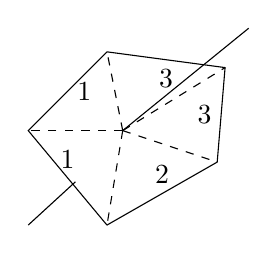
\begin{tikzpicture}	
	\draw (0,0) --node[above]{$2$} (1.4,0.8) -- node[left]{$3$} (1.5,2) -- node[below]{$3$}(0,2.2) -- node[right]{$1$}(-1,1.2) --node[above]{$1$} (0,0);
	
	\draw (0.2,1.2) -- (1.8,2.5);
	\draw (-0.4,0.55) -- (-1,0);
	\draw[dashed] (0.2,1.2) -- (0,0);
	\draw[dashed] (0.2,1.2) -- (1.4,0.8);
	\draw[dashed] (0.2,1.2) -- (1.5,2);
	\draw[dashed] (0.2,1.2) -- (0,2.2);
	\draw[dashed] (0.2,1.2) -- (-1,1.2);
\end{tikzpicture}

\end{figure*}


\item  A card is dealt from a well-shuffled ordinary pack of $52$ playing cards.
\begin{enumerate}
	\item Find the probability that the card is 
	\begin{enumerate}
		\item the $3$ of the spades,
		\item the $3$ of the spades or any diamond.
	\end{enumerate}
\item The first card dealt is placed face-up on the table. It is the $3$ of diamonds. What is the probability that the second card is from a red suit?
\end{enumerate}


\item The table shows the results of all the driving tests taken at a particular test centre during the first week of September. A person is chosen at random from those who took their driving test that week.
\begin{center}

		\begin{tabular}{l|c|c|}
			\cline{2-3}
			& \textbf{Male} & \textbf{Female} \\ \hline
			\multicolumn{1}{|l|}{\textbf{Pass}} & 32            & 43              \\ \hline
			\multicolumn{1}{|l|}{\textbf{Fail}} & 10            & 15              \\ \hline
		\end{tabular}

\end{center}


\begin{enumerate}
	\item Find the probability that the person passed the driving test.
	\item Find the probability that the person is a female who failed the driving test.
	\item A male is chosen. What is the probability that he passed  the driving test.
\end{enumerate}


\item An ordinary tetrahedral die has four faces and they are labelled $1$, $2$, $3$, $4$. When 	the die is thrown, the score is the number on which the die lands. Two fair tetrahedral dice are thrown. By using a possibility space diagram, or otherwise, find the probability that 
\begin{enumerate}
	\item the sum of the scores is divisible by $4$,
	\item the product of the scores is an even number,
	\item the scores differ by at least $2$. 
\end{enumerate} 

\item Two fair coins are tossed together. Find the probability that

\begin{enumerate}
	\item exactly one tail is obtained,
	\item at most one head is obtained.
\end{enumerate}

\item Two ordinary fair cubical dice are thrown. Find the probability that 

\begin{enumerate}
	\item the sum of the numbers on the dice is $3$,
	\item the sum of the numbers on the dice exceeds $9$,
	\item the dice show the same number,
	\item the numbers on the dice differ by more than 2.
\end{enumerate}

\item Two ordinary fair cubical dice are thrown at the same time and the scores are multipled. $\text{P}(N)$ denotes the probability that the number $N$ will be obtained.

\begin{enumerate}
	\item Find 
	\begin{enumerate}
		\item $\text{P}(9)$,
		\item $\text{P}(4)$,
		\item $\text{P}(14)$,
		\item $\text{P}(37)$.
	\end{enumerate}
\item If $\text{P}(N) = \frac{1}{9}$, find the possible values of $N$.
\end{enumerate}

\item Three fair coins are tossed,
\begin{enumerate}
	\item List all possible outcomes,
	\item Find the probability that two heads and one tail are obtained.
\end{enumerate}




\end{enumerate}

\newpage

\subsection{Using permutations and combinations}
%%%%%%%%%%%%%%%%%%%%%%%%%%%%%%%%%%%%%%%%%%%%%
%%%%%%%%%%%%%%%%%%%%%%%%%%%%%%%%%%%%%%%%%%%%%
%%%%%%%%%%%%%%%%%%%%%%%%%%%%%%%%%%%%%%%%%%%%%
%%%%%%%%%%%%%%%%%%%%%%%%%%%%%%%%%%%%%%%%%%%%%
%% 3.2 Using permutations and combinations %%%
%%%%%%%%%%%%%%%%%%%%%%%%%%%%%%%%%%%%%%%%%%%%%
%%%%%%%%%%%%%%%%%%%%%%%%%%%%%%%%%%%%%%%%%%%%%
%%%%%%%%%%%%%%%%%%%%%%%%%%%%%%%%%%%%%%%%%%%%%
%%%%%%%%%%%%%%%%%%%%%%%%%%%%%%%%%%%%%%%%%%%%%
%\setlength\itemsep{0.5em}

In order to find the number of outcomes in a particular event and in the possibility space, you may need to use arrangements permutations and combinations.


\exercise  %%%% --- Exercise 14


\begin{enumerate}
	\item Evan throws three fair dice.
	\begin{enumerate}
		\item List all possible scores on the three dice which give a total of $5$,  and hence show that the probability of Evan obtaining a total score of $5$ is $\frac{1}{36}$.
		\item Find the probability of Evan obtaining a total score of $7$.
	\end{enumerate}

   \item Each of the eleven letters of the word \textbf{MATHEMATICS} is written on a separate card and cards are laid out in a line.
   
   \begin{enumerate}
   	\item Calculate the number of different arrangements of these letters.
   	\item Find the probability that all the vowels are placed together.
   \end{enumerate}


\item Four letters are chosen at random from the letters in the word \textbf{RANDOMLY}. Find the probability that all letters chosen are consonants.

\item A team of $5$ pupils is chosen from a class of $7$ girls and $8$ boys. Find the probability that the team consists of $3$ girls and $2$ boys.

\item  A staff park at a school has $13$ parking spaces in a row.  There are $9$ cars to be parked.
\begin{enumerate}
	\item How many different arrangements are there for parking the $9$ cars and leaving $4$ empty spaces?
	\item How many different arrangements are there if the $4$ empty spaces are next to each other?
	\item If the parking is random, find the probability that there will not be $4$ empty spaces next to each other?
\end{enumerate}


\item  Minerva is given a bag of $20$ sweets of which $6$ are apple flavoured , $6$ are lemon flavoured and $8$ are orange flavoured. Minerva takes out $5$ sweets at random and eats them. Find the probability that she eats:
\begin{enumerate}
	\item $5$ orange flavoured sweets,
	\item $3$ apple flavoured and $2$ lemon flavoured sweets,
	\item exactly $2$ apple flavoured sweets,
	\item no lemon flavoured sweets. 
\end{enumerate}

\item  A plate contains $15$ cakes of which $6$ have yellow icing, $5$ have green icing and $4$ have pink icing.  Three cakes are taken at random from the plate.

Find the probability that:

\begin{enumerate}
	\item exactly two of the cakes have green icing,
	\item one cake has green icing, one has pink icing and one has yellow icing,
	\item none of the cakes has yellow icing.
\end{enumerate}


\item Peter deals a hand of $10$ cards from a well-shuffled pack of ordinary playing cards.	Show the probability that she deals exactly $5$ spades is less than $5\%$.







\end{enumerate}




\newpage

\subsection{Two or more events}
%%%%%%%%%%%%%%%%%%%%%%%%%%%%%%%%%%%%%%%%%%%%%
%%%%%%%%%%%%%%%%%%%%%%%%%%%%%%%%%%%%%%%%%%%%%
%%%%%%%%%%%%%%%%%%%%%%%%%%%%%%%%%%%%%%%%%%%%%
%%%%%%%%%%%%%%%%%%%%%%%%%%%%%%%%%%%%%%%%%%%%%
%%%%%%%% 3.3 Two or more events %%%%%%%%%%%
%%%%%%%%%%%%%%%%%%%%%%%%%%%%%%%%%%%%%%%%%%%%%
%%%%%%%%%%%%%%%%%%%%%%%%%%%%%%%%%%%%%%%%%%%%%
%%%%%%%%%%%%%%%%%%%%%%%%%%%%%%%%%%%%%%%%%%%%%
%%%%%%%%%%%%%%%%%%%%%%%%%%%%%%%%%%%%%%%%%%%%%
%\setlength\itemsep{0.5em}


Now consider two events, $A$ and $B$, in the possibility tree.

\medskip


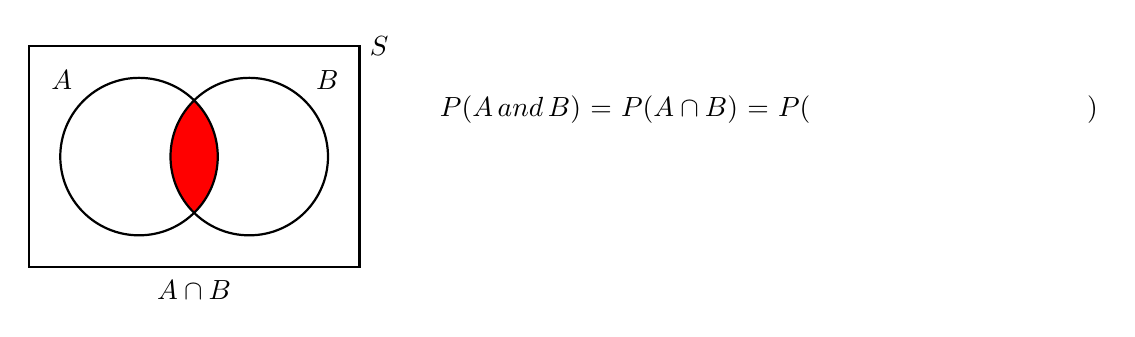
\begin{tikzpicture}[thick,
	set/.style = {circle,
		minimum size = 2cm,
		fill=white}]
	
	% Set A
	\node[set,label={135:$A$}] (A) at (0,0) {};
	
	% Set B
	\node[set,label={45:$B$}] (B) at (1.4,0) {};
	
	% Intersection
	\begin{scope}
		\clip (0,0) circle(1cm);
		\clip (1.4,0) circle(1cm);
		\fill[red](0,0) circle(1cm);
	\end{scope}
	
	% Circles outline
	\draw (0,0) circle(1cm);
	\draw (1.4,0) circle(1cm);
	
	% Set intersection label
	\node at (0.7,-1.7) {$A\cap B$};
	
	\draw (-1.4, -1.4) rectangle (2.8,1.4) node[right]{$S$};
	
	
	\node at (8,0.6) {$\text{P}(A \,\text{and} \, B)$ = $\text{P}(A\cap B)$ = $\text{P}(\qquad \qquad \qquad  \qquad \qquad  )$};
	
\end{tikzpicture}


\medskip

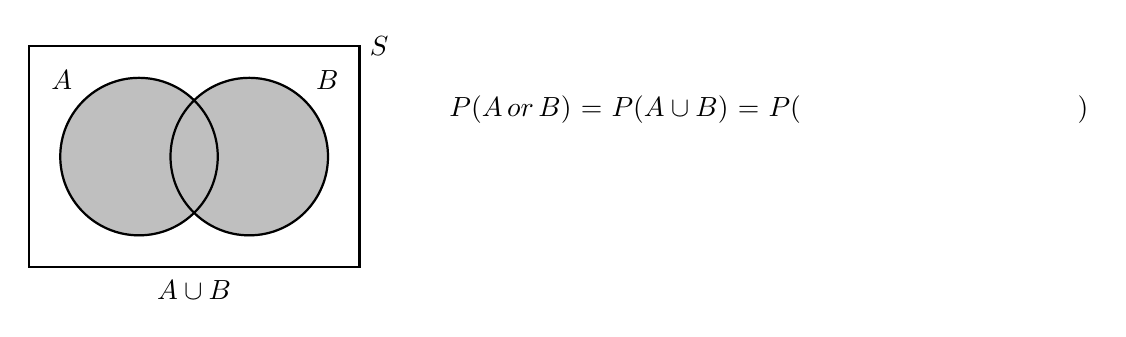
\begin{tikzpicture}[thick,
	set/.style = {circle,
		minimum size = 2cm,
		fill=white}]
	
	% Set A
	\node[set,label={135:$A$}] (A) at (0,0) {};
	
	% Set B
	\node[set,label={45:$B$}] (B) at (1.4,0) {};
	
	% Intersection
%	\begin{scope}
%		\clip (0,0) circle(1cm);
%		\clip (1.4,0) circle(1cm);
%		\fill[red](0,0) circle(1cm);
%	\end{scope}
	
	% Circles outline
	\filldraw[lightgray] (0,0) circle(1cm);
	\filldraw[lightgray] (1.4,0) circle(1cm);
	
		% Circles outline
	\draw (0,0) circle(1cm);
	\draw (1.4,0) circle(1cm);
	
	% Set intersection label
	\node at (0.7,-1.7) {$A\cup B$};
	
	\draw (-1.4, -1.4) rectangle (2.8,1.4) node[right]{$S$};
	
	
	\node at (8,0.6) {$\text{P}(A \,\text{or} \, B)$ = $\text{P}(A\cup B)$ = $\text{P}(\qquad \qquad \qquad  \qquad \qquad  )$};
	
\end{tikzpicture}


\medskip

Addition rule for combined events:

\[
\text{P}(A\, \text{or} \, B) = \text{P}(A) +  \text{P}(B) - \text{P}(A\,\text{and}\, B).
\]

Using set notation:

\[
\text{P}(A\cup  B) = \text{P}(A) +  \text{P}(B) - \text{P}(A \cap B).
\]


\exercise  %%%  -- Exercise 15

\begin{enumerate}
	\item Two events, $X$ and $Y$, are such that $\text{P}( X \, \text{or} \, Y) =0.8$, $\text{P}( X \, \text{and} \, Y) =0.35$ and $\text{P}( X ) =0.6$. Find $\text{P}(Y') $.
	
	\item Events $A$ and $B$ are such that $\text{P}(A \,\text{occurs})=0.6$,  $\text{P}(B \,\text{occurs})=0.7$, $\text{P}(\text{at least one of}\, A \, \text{and}\, B \, \text{occurs})=0.9$.
	
	Find 
	\begin{enumerate}
		\item $\text{P}(\text{both}\, A \, \text{and}\, B \, \text{occur})$.
		\item $\text{P}(\text{neither}\, A \, \text{and}\, B \, \text{occurs})$.
		\item $\text{P}( A \, \text{occurs or}\, B \, \text{occurs but not both} \, A \, \text{and}\, B \, \text{occurs})$
	\end{enumerate}
	
	
	\item   Some pupils did a survey on comics. They asked all $100$ pupils in theri year group whether they read particular comics during the past week. They found that $65$ had read Whizz, $55$ had read Wham, $30$ had read Whizz and Wham and some pupils  in the year group had not read either comic.
	
	A pupil was selected at random from the year group to answer more questions in the survey. Find the probability that the pupil
	
	\begin{enumerate}
		\item had read Whizz or Wham,
		\item had not read either comic.
	\end{enumerate}




\end{enumerate}

\newpage

\textbf{Mutually exclusive events}

\medskip

Events are mutually exclusive $\underline{\text{if they cannot occur at the same time.}}$

\medskip


For example, with one throw of a die, the events 'scoring a $3$' and 'scoring a $5$' are mutually exclusive, since the score cannot be $3$ and $5$ at the same time. 

\medskip 
However, the events 'scoring an even number' and 'scoring a prime number' are not mutually exclusive, since a score of $2$ is both even and prime.


\medskip

\medskip 

Set notation and Venn diagram:

\medskip

When $A$ and $B$ are mutually exclusive there is no overlap between $A$ and $B$.

\begin{figure*}[!htpb]
	\centering
	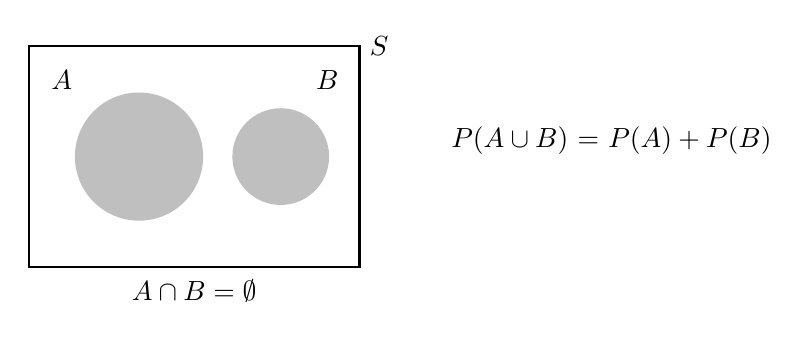
\begin{tikzpicture}[thick,
		set/.style = {circle,
			minimum size = 2cm,
			fill=white}]
		
		% Set A
		\node[set,label={135:$A$}] (A) at (0,0) {};
		
		% Set B
		\node[set,label={45:$B$}] (B) at (1.4,0) {};
		
		% Intersection
		%	\begin{scope}
		%		\clip (0,0) circle(1cm);
		%		\clip (1.4,0) circle(1cm);
		%		\fill[red](0,0) circle(1cm);
		%	\end{scope}
		
		% Circles outline
		\filldraw[lightgray] (0,0) circle(0.8cm);
		\filldraw[lightgray] (1.8,0) circle(0.6cm);
		
		% Circles outline
		%	\draw (0,0) circle(1cm);
		%	\draw (1.4,0) circle(1cm);
		
		% Set intersection label
		\node at (0.7,-1.7) {$A\cap B = \emptyset$};
		
		\draw (-1.4, -1.4) rectangle (2.8,1.4) node[right]{$S$};
		
		
		\node at (6,0.2) {$\text{P}(A\cup B)$ = $\text{P}(A) +  \text{P}(B)$};
		
	\end{tikzpicture}

\end{figure*}

\medskip

Note: if you are asked to show that event $A$ and event $B$ are mutually exclusive, you must give working  to show either the following is satisfied:

\[
\text{P}(A\cup B) = \text{P}(A) +  \text{P}(B) \qquad  \qquad \text{P}(A \cap B) =0.
\]

\exercise  %%%% --------- Exercise 16


\begin{enumerate}
	\item  In a race where there can be only one winner, the probability that John will win is $0.3$,  the probability that Paul will win is $0.2$ and the probability that Mark will win is $0.4$.
	
	Find the probabilibty that 
	
	\begin{enumerate}
		\item John or Mark wins,
		\item John or Paul or Mark wins,
		\item someone else wins.
	\end{enumerate}

\item  A card is dealt from an ordinary pack of $52$ playing cards. Find the probability that the card is 
\begin{enumerate}
	\item a club or a diamond,
	\item a club or a king.
\end{enumerate}

\item Two fair dice are shown.
\begin{enumerate}
	\item Event $A$ is 'the scores differ by $3$ or more'. Find the probability of event $A$.
	\item Event $B$ is 'the product of the scores is greater than $8$'. Find the probability of event $B$.
	\item State with a reason whether events $A$ and $B$ are mutually exclusive.
\end{enumerate}
	
	
	
	
	\item Two fair cubical dice are thrown.
	
	Event $A$ is 'the scores on the dice are the same',
	
	Event $B$ is 'the product of the scores is a multiple of $3$',
	
	Event $C$ is 'the sum of the scores is $7$'.
	
	State with a reason whether $A$ and $B$, $A$ and $C$, $B$ and $C$ are mutually exclusive.
	
	
	
	
\end{enumerate}


\newpage

\subsection{Condtional probability}
%%%%%%%%%%%%%%%%%%%%%%%%%%%%%%%%%%%%%%%%%%%%%
%%%%%%%%%%%%%%%%%%%%%%%%%%%%%%%%%%%%%%%%%%%%%
%%%%%%%%%%%%%%%%%%%%%%%%%%%%%%%%%%%%%%%%%%%%%
%%%%%%%%%%%%%%%%%%%%%%%%%%%%%%%%%%%%%%%%%%%%%
%%%%%%%% 3.4 Conditional probability %%%%%%%%%%%
%%%%%%%%%%%%%%%%%%%%%%%%%%%%%%%%%%%%%%%%%%%%%
%%%%%%%%%%%%%%%%%%%%%%%%%%%%%%%%%%%%%%%%%%%%%
%%%%%%%%%%%%%%%%%%%%%%%%%%%%%%%%%%%%%%%%%%%%%
%%%%%%%%%%%%%%%%%%%%%%%%%%%%%%%%%%%%%%%%%%%%%
%\setlength\itemsep{0.5em}

Condtional probability is used when the probability that an event will occur depends on whether another event has happened.

\medskip

For event $A$ and $B$, the conditional probability that event $B$ occurs, given that $A$ has already occured, i.e.
\[
\text{P}(B \, \text{given}\, A) = \text{P}(B|A)
\]


\medskip
\begin{figure*}[!htpb]
	\centering
	\begin{tikzpicture}[thick,
		set/.style = {circle,
			minimum size = 2cm,
			fill=white}]
		
		% Set A
		\node[set,label={135:$A$}] (A) at (0,0) {};
		
		% Set B
		\node[set,label={45:$B$}] (B) at (1.4,0) {};
		
		
		\filldraw[lightgray] (0,0) circle(1cm);
		% Intersection
		\begin{scope}
			\clip (0,0) circle(1cm);
			\clip (1.4,0) circle(1cm);
			\fill[red](0,0) circle(1cm);
		\end{scope}
		
		% Circles outline
		\draw (0,0) circle(1cm);
		\draw (1.4,0) circle(1cm);
		
		% Set intersection label
		\node at (0.7,-1.7) {$A\, \text{and}\, B$};
		
		\draw (-1.4, -1.4) rectangle (2.8,1.4) node[right]{$S$};
		
		
		\node at (8,0.1) {$\begin{aligned}
				\text{P}(B|A) &= \frac{n(A \, \text{and} \,B )}{n(A)}
				&= \frac{\frac{n(A \, \text{and} \,B )}{\quad}}{\frac{n(A)}{\quad }} 
				& = \frac{\text{P}(A \,\text{and}\, B)}{\text{P}(A)}.\\
			\end{aligned}$};
		
	\end{tikzpicture}
\end{figure*}

This gives the multiplication rule:

\[
\text{P}(A \,\text{and}\, B) =  \text{P}(A) \times  \text{P}(\qquad ).
\]

\exercise  %%   %%%%%%%%%%%% -- Exercise 17

\begin{enumerate}
	\item There are $5$ red counters and $7$ blue counters in a bag. Darian takes  a counter from the bag, puts it on the table and then takes another counter from the bag. Find the probability  that he takes out
	
	\begin{enumerate}
		\item a red counter then a blue counter,
		\item two counters that are the same colour,
		\item at least one red counter.
	\end{enumerate} 


  \item  Two events $X$ and $Y$ are such that $\text{P}(X)=0.2$,  $\text{P}(Y)=0.25$,  $\text{P}(Y|X)=0.4$.
  
  Find 

  \begin{enumerate*}
  	\item $\text{P}(X \,\text{and}\, Y)$,\qquad \,
  	
  	\item $\text{P}(X|Y)$, \qquad \,
  	
  	\item $\text{P}(X \,\text{or}\, Y)$.
  \end{enumerate*}


\item Of the $120$ first year students at a college, $36$ study chemistry, $60$ study biology and $10$ study both chemistry and biology. A first year student is selected at random to represent the college at a conference. Find the probability that the student studies
\begin{enumerate}
	\item chemistry, given that the student studie biology,
	\item biology, given that the student studies  chemistry.
\end{enumerate}

\item Last month a consultant saw $60$ men and $65$ women suspected  of having a particular eye condition. Tests were carried out and the following table shows the results. The totals are shown in bold.

\begin{table}[!htpb]
	\centering
	\begin{tabular}{l|c|c|c}
		\cline{2-3}
		& \textbf{Had eye condition (C)} & \textbf{Did not have eye condition (C')} &                                   \\ \hline
		\multicolumn{1}{|l|}{\textbf{Man (M)}}   & 25                             & 35                                       & \multicolumn{1}{c|}{\textbf{60}}  \\ \hline
		\multicolumn{1}{|l|}{\textbf{Woman (W)}} & 20                             & 45                                       & \multicolumn{1}{c|}{\textbf{65}}  \\ \hline
		& \textbf{45}                    & \textbf{80}                              & \multicolumn{1}{c|}{\textbf{125}} \\ \cline{2-4} 
	\end{tabular}
\end{table}

One of these  patients was selected at random to take part in a survey. Find the probability that the patient selected
\begin{enumerate}
	\item was a women, given that the patient had the eye condition
	\item had the eye condition, given that the patient was a man.
\end{enumerate}




\end{enumerate}

\newpage

\textbf{Independent events}

\medskip

In general, the following rule is correct for any events $A$ and $B$

\[
\text{P}(A \,\text{and}\, B) =  \text{P}(A) \times  \text{P}(B|A).
\]

Now when either of these events can occur without being affected by the outcome of the other,	the events 	are said to be $\underline{\hspace{3cm}}$.

\medskip

So, for \textbf{independent events} $A$ and $B$,

\[
 \text{P}(B|A) = \text{P}(\quad )
\] 
Also

\[
\text{P}(A|B) = \text{P}(\quad )
\]

This gives the multiplication rule for \textbf{independent events}:

\[
\text{P}(A \,\text{and}\, B) =  \text{P}(A) \times  \text{P}(B).
\]

In set notation

\[
\text{P}(\qquad\quad ) =  \text{P}(A) \times  \text{P}(B).
\]

\exercise  %%%%%%%%%%%% --- Exercise 18

\begin{enumerate}
	\item There are $5$ red counters and $7$ blue counters in a bag. Eliza takes a  counter from the bag, notes its colour and then puts it back into the bag. Freddie then takes a counter from the bag. Find the probability that
	\begin{enumerate}
		\item Eliza takes a red counter and Freddie  takes a blue counter,
		\item Freddie's counter is the same colour as Eliza's counter.
	\end{enumerate}


\item Two fair cubical dice are thrown. One is red and the other is blue. Find the probability that 

\begin{enumerate}
	\item the score is $3$ on both dice,
	\item neither die has a score of $3$.
\end{enumerate}


\item The probability that a certain type of machine will break down in the first month of operation is $0.1$. Three machines of this type are installed at the same time. The performances of the three machines are independent. Find the probability that at the end of the first month
\begin{enumerate}
	\item all three machines have broken down,
	\item just one machine has broken down,
	\item at least one machine is working.
\end{enumerate}

\item In a large group of people it is known that $10\%$ have a hot breakfast, $20\%$ have a hot lunch and $25\%$ have a hot breakfast or a hot lunch. Find the probability that a person chosen at random from this group

\begin{enumerate}
	\item has a hot breakfast and a hot lunch.
	\item has a hot lunch, given that the person chosen had a hot breakfast.
\end{enumerate}

\item Two events $A$ and $B$ are such that $\text{P}(A|B) =0.4$, $\text{P}(B|A) =0.25$ and $\text{P}(A \,\text{and} \, B) =0.12$.

\begin{enumerate}
	\item Are $A$ and $B$ independent? Give a reason for your answer.
	\item Find $\text{P}(A \,\text{or} \,B)$.
\end{enumerate}

\newpage 

\item Data about employment for males and females in a small rural area are shown in the table.



\begin{table}[!htpb]
	\centering
	\begin{tabular}{l|c|c|}
		\cline{2-3}
		& \textbf{Unemployed} & \textbf{Employed} \\ \hline
		\multicolumn{1}{|l|}{\textbf{Male}}   & 206                 & 412               \\ \hline
		\multicolumn{1}{|l|}{\textbf{Female}} & 358                 & 305               \\ \hline
	\end{tabular}
\end{table}




A person from this area is chosen at random. Let $M$ be the event that the person is male and let $E$ be the event that the person is employed.

\begin{enumerate}
	\item Find $\text{P}(M)$.
	\item Find $\text{P}(M\,\text{and}\, E)$.
	\item Are $M$ and $E$ independent events? Justify your answer.
	\item 	Given that the person chosen is unemployed, find the probability  that the person is female.
\end{enumerate}






\item Two ordinary fair dice, one red and one blue, are thrown.

Events $A$, $B$ and $C$ are defined as follows:

Event $A$: the number showing on the red die is $5$ or $6$

Event $B$: the total of the numbers showing on the two dice is $7$

Event $C$: the total of the numbers showing on the two dice is $8$

\begin{enumerate}
	\item State, with a reason, which two of the events $A$, $B$ and $C$ are mutually exclusive.
	\item Show that the events $A$ and $B$ are independent.
\end{enumerate}




\item A school has $100$ teachers. In a survey on the use of the school car park, the teachers were asked 	whether they had driven a car to school on a particular day. Of the $70$ full-time teachers, 	$45$ had driven a car to  school and of the $30$ part-time teachers, $12$ had driven a car to school.

\begin{enumerate}
	\item Copy and complete the two-way table, where $C$ denotes the event 'the teacher had driven  a car to school that day'.
	
	\begin{table}[!htpb]
		\centering
		\begin{tabular}{r|c|c|c}
			\cline{2-3}
			& \, \,C \, \, & \, \, C'\,\, & Total                    \\ \hline
			\multicolumn{1}{|r|}{Full-time teacher} &   &    & \multicolumn{1}{c|}{}    \\ \hline
			\multicolumn{1}{|r|}{Part-time teacher} &   &    & \multicolumn{1}{c|}{}    \\ \hline
			Total                                   &   &    & \multicolumn{1}{c|}{100} \\ \cline{2-4} 
		\end{tabular}
	\end{table}
	
	\item Find the probability that a teacher chosen at random
	\begin{enumerate}
		\item is a part-time teacher who had driven a car to school,
		\item is a full-time teacher who had not driven a car to school,
		\item is a full-time teacher or had driven 	a car to school,
		\item is a part-time teacher, given that the teacher had driven a car to school.
	\end{enumerate}

\item Are the events 'the teacher had driven a car to school' and 'the teacher is full-time' independent? Give a reason for your answer.
\item Describe two events that are mutally exclusive.    
	
	
\end{enumerate}
 


\end{enumerate}

\newpage

\subsection{Probability trees}
%%%%%%%%%%%%%%%%%%%%%%%%%%%%%%%%%%%%%%%%%%%%%
%%%%%%%%%%%%%%%%%%%%%%%%%%%%%%%%%%%%%%%%%%%%%
%%%%%%%%%%%%%%%%%%%%%%%%%%%%%%%%%%%%%%%%%%%%%
%%%%%%%%%%%%%%%%%%%%%%%%%%%%%%%%%%%%%%%%%%%%%
%%%%%%%% 3.5 Probability trees %%%%%%%%%%%
%%%%%%%%%%%%%%%%%%%%%%%%%%%%%%%%%%%%%%%%%%%%%
%%%%%%%%%%%%%%%%%%%%%%%%%%%%%%%%%%%%%%%%%%%%%
%%%%%%%%%%%%%%%%%%%%%%%%%%%%%%%%%%%%%%%%%%%%%
%%%%%%%%%%%%%%%%%%%%%%%%%%%%%%%%%%%%%%%%%%%%%
%\setlength\itemsep{0.5em}

A very useful method for tacking many probability problems is to draw a tree diagram. 

\medskip

For example,  a jar contains seven red discs and four white discs. Two disc are selected without replacement.
 
\medskip
A tree diagram can be formed as follows:

\begin{figure*}[!htpb]
	\centering
	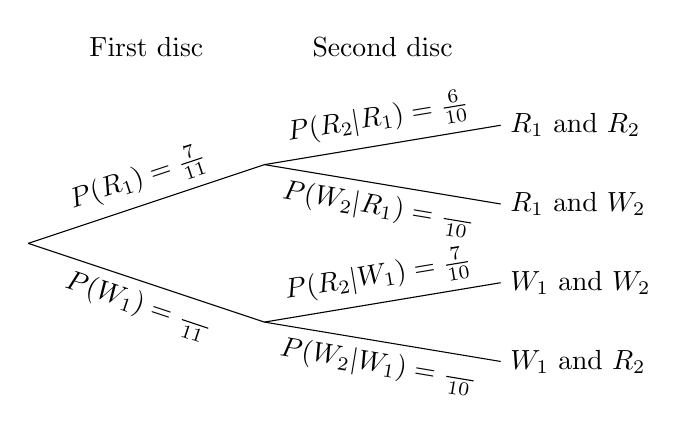
\begin{tikzpicture}
		\draw (0,0) --node[midway,rotate=atan(1/3),above]{$\text{P}(R_1) = \frac{7}{11}$}(3,1) --node[midway,rotate=atan(1/6),above]{$\text{P}(R_2|R_1) = \frac{6}{10}$} (6,1.5) node[right]{$R_1$ and $R_2$};
		\draw         (3,1) --node[midway,rotate=-atan(1/6),below]{$\text{P}(W_2|R_1) = \frac{\quad}{10}$} (6,0.5) node[right]{$R_1$ and $W_2$};
		
		
		
		\draw (0,0) --node[midway,rotate=atan(-1/3),below]{$\text{P}(W_1) = \frac{\quad }{11}$}(3,-1) --node[midway,rotate=-atan(1/6),below]{$\text{P}(W_2|W_1) = \frac{\quad}{10}$} (6,-1.5) node[right]{$W_1$ and $R_2$};
		\draw         (3,-1) -- node[midway,rotate=atan(1/6),above]{$\text{P}(R_2|W_1) = \frac{7}{10}$}(6,-0.5) node[right]{$W_1$ and $W_2$};
		
		\node[] (A) at (1.5,2.5) {First disc};
		
		\node[] (A) at (4.5,2.5) {Second disc};
		
	\end{tikzpicture}
\end{figure*}

then you can find the probability that both of the discs are red by:

\[
\text{P}(R_1\,\text{and}\, R_2) = \text{P}(R_1) \times \text{P}(R_2|R_1) = \qquad  \times \qquad = \qquad .
\]

Meanwhile, the probability of the second discs is red is given by:

\[
\text{P}(R_2) = \text{P}(\qquad \,\text{and}\, R_2) + \text{P}(\qquad \,\text{and}\, R_2) = 
\]


\exercise %%%  -----Exercise 19
 
\begin{enumerate}
	\item In a country $A$ $30\%$ of people who drink tea have sugar in it. In country $B$ $65\%$ of people who drink tea have sugar in it. There are $3$ million in country $A$ who drink tea and $12$ million in country $B$ who drink tea.  A person is chosen at random from these $15$ million people.
	\begin{enumerate}
		\item Find the probability that the person chosen is from country $A$.
		\item Find the probability that the person chosen does not have sugar in their tea.
		\item Given that chosen does not have sugar in their tea, find the probability that the person is from country $B$.
	\end{enumerate}
	
	\item  There are three sets of traffic lights on Karinne's journey to work. The independent probabilities that Karinne has to stop at the first, second and third sets of lights are $0.4$, $0.8$ and $0.3$ respectively.
	\begin{enumerate}
		\item Draw a tree diagram to show this information.
		\item Find the probability that Karinne has to stop at each of the first two sets of lights but does not have to stop at the third set of lights.
		\item Find the probability that Karinne has to stop at exactly two of the three sets of lights.
		\item Find the probability that Karinne has to stop at the first set of lights, given that she has to stop at exactly two sets of lights.
	\end{enumerate}

\item Dan is playing a game in which players pick counters at random, one at a time without replacement, from a bag. At the beginning of the game, the bag contains $6$ red counters and $4$ blue counters. Dan takes two counters from the bag.

\begin{enumerate}
	\item Find the probability that both counters are blue.
	\item Find the probability that the counters are the same color.
	\item Given that the counters are the same color, find the probability that they are both blue.
\end{enumerate} 
	
	
	
	\item When a farmer's dog is let loose, it chases either ducks with probability $\frac{3}{5}$ or geese with probability $\frac{2}{5}$. If the dog chases the ducks, there is a probability of $\frac{1}{10}$ that they will attack the dog. If the dog chases the geese, there is a probability of $\frac{3}{4}$ that they will attack the dog. Given that the dog is not attacked, find the probability that it was chasing the geese. 
	
	
	\item  The probability that Henk goes swimming on any day is $0.2$. On a day that he goes swimming, the probability that Henk has burgers for supper is $0.75$. On a day when he does not go swimming, the probability that he has burgers for his supper is $x$.  The information is shown on the following tree diagram.
	
	\begin{figure*}[!htpb]
		\centering
		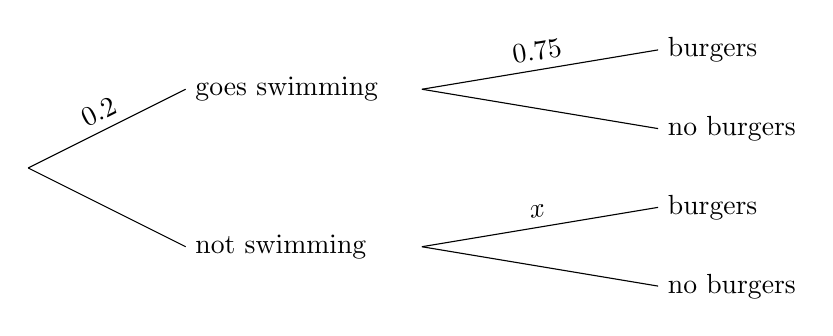
\begin{tikzpicture}
			\draw (0,0) --node[midway,rotate=atan(1/2),above]{$0.2$}(2,1) node[right]{goes swimming};
			
			\draw         (5,1) --node[midway,rotate=atan(1/6),above]{$0.75$} (8,1.5) node[right]{burgers};
			
			\draw         (5,1) -- (8,0.5) node[right]{no burgers};
			
			\draw (0,0) --(2,-1) node[right]{not swimming};
			
			\draw         (5,-1) --node[midway,rotate=atan(1/6),above]{$x$} (8,-0.5) node[right]{burgers};
			
			\draw         (5,-1) -- (8,-1.5) node[right]{no burgers};
	
		\end{tikzpicture}
	\end{figure*}
	
	The probability that Henk has burgers for supper on any day is $0.5$.
	\begin{enumerate}
		\item Find $x$.
		\item Given that Henk has burgers for supper, find the probability that he went swimming that day.
	\end{enumerate}
	
	
	
	\item When Don plays tennis, $65\%$ of his first serves go into the correct are of the court. If the first serve goes into the correct area, his chance of winning the point is $90\%$. If his first serve does not go into the correct area, Don is allowed a second serve and, of these, $80\%$ go into the correct area. If the second serve goes into the correct, his chance of winning the point is $60\%$. If neither serve goes into the correct area, Don loses the point.
	\begin{enumerate}
		\item Draw a tree diagram to represent  this information.
		\item Using the tree diagram, find the probability that Don loses the point.
		\item Find the conditional probability that Don's first serve went into the correct area, given that he loses the point.
	\end{enumerate} 
	
	
	
	\item In an archery competition, Bill is allowed up to three attempts to hit the target. If he succeeds on any attempt, he does not make any more attempts. The probability that he will hit the target on the first attempt is $0.6$. If he misses, the probability that he will hit the target on his second attempt is $0.7$. If he misses on the second attempt, the probability that he will hit the target on his third attempt is $0.8$.
	
	\begin{enumerate}
		\item Draw a fully labelled tree diagram.
		\item Find the probability that Bill will hit the target.
		\item Given that Bill hits the target, find the probability that he made at least two attempts.
	\end{enumerate}


\item Boxes of sweets contain toffees and chocolates. Box $A$ contains $6$ toffees and $4$ chocolates, box $B$ contains $5$ toffees and $3$ chocolates and box $C$ contains $3$ toffees and $7$ chocolates. One of the boxes is chosen at random and two sweets are taken out, one after the other, and eaten.
\begin{enumerate}
	\item Find the probability that they are both toffees.
	\item Given that they are both toffees, find the probability that they both came from box $A$.
\end{enumerate}
	
	
\end{enumerate}	
	
	\newpage
	
	
	
	\mis     %%%%%%%% Miscelaneous 3
	
	\begin{enumerate}
		
		
	%%%%%%%%%%%%%%%%%%%%%%%%%%%%%%%%%%	
	%%%%%%%%%%%%%%%%%%%%%%%%%%%%%%%%%%	
	%%%%%%%%%%%%%%%%%%%%%%%%%%%%%%%%%%	
	%%%%    Q1 m17_qp_62  q2      %%%	
	%%%%%%%%%%%%%%%%%%%%%%%%%%%%%%%%%%	
	%%%%%%%%%%%%%%%%%%%%%%%%%%%%%%%%%%	
	%%%%%%%%%%%%%%%%%%%%%%%%%%%%%%%%%%
		
		\item A bag contains $10$ pink balloons, $9$ yellow balloons, $12$ green balloons and $9$ white balloons. $7$ balloons are selected at random without replacement. Find the probability that exactly $3$ of them are green.  \hfill [3]
		
		
%%%%%%%%%%%%%%%%%%%%%%%%%%%%%%%%%%	
%%%%%%%%%%%%%%%%%%%%%%%%%%%%%%%%%%	
%%%%%%%%%%%%%%%%%%%%%%%%%%%%%%%%%%	
%%%%    Q2 m18_qp_62  q3      %%%	
%%%%%%%%%%%%%%%%%%%%%%%%%%%%%%%%%%	
%%%%%%%%%%%%%%%%%%%%%%%%%%%%%%%%%%	
%%%%%%%%%%%%%%%%%%%%%%%%%%%%%%%%%%		

\item Last Saturday, Sarah recorded the colour and type of $160$ cars in a car park. All the cars that were not red or silver in colour were grouped together as 'other'. Her results are shown in the following table.

	\begin{table}[!htpb]
		\centering
		\begin{tabular}{ll|ccc|}
			\cline{3-5}
			\multicolumn{1}{c}{}                                &        & \multicolumn{3}{c|}{Type of Car}                                      \\ \cline{3-5} 
			\multicolumn{1}{c}{}                                &        & \multicolumn{1}{c|}{Saloon} & \multicolumn{1}{c|}{Hatchback} & Estate \\ \hline
			\multicolumn{1}{|l|}{\multirow{3}{*}{Color of car}} & Red    & \multicolumn{1}{c|}{20}     & \multicolumn{1}{c|}{40}        & 12     \\ \cline{2-5} 
			\multicolumn{1}{|l|}{}                              & Silver & \multicolumn{1}{c|}{14}     & \multicolumn{1}{c|}{26}        & 10     \\ \cline{2-5} 
			\multicolumn{1}{|l|}{}                              & Other  & \multicolumn{1}{c|}{6}      & \multicolumn{1}{c|}{24}        & 8      \\ \hline
		\end{tabular}
	\end{table}

\begin{enumerate}
	\item Find the probability that a randomly chosen car in the car park is a silver estate car. \hfill [1]
	\item Find the probability that a randomly chosen car in the car park is a hatchback car. \hfill[1]
	\item Find the probability that a randomly chosen car in the car park is red, given that it is a hatchback
	car.\hfill [2]
	\item  One of the cars in the car park is chosen at random. Determine whether the events 'the car is a hatchback car' and 'the car is red' are independent, justifying your answer. \hfill [2]
\end{enumerate}
		
		
		
		
%%%%%%%%%%%%%%%%%%%%%%%%%%%%%%%%%%	
%%%%%%%%%%%%%%%%%%%%%%%%%%%%%%%%%%	
%%%%%%%%%%%%%%%%%%%%%%%%%%%%%%%%%%	
%%%%    Q3 s17_qp_61  q2      %%%	
%%%%%%%%%%%%%%%%%%%%%%%%%%%%%%%%%%	
%%%%%%%%%%%%%%%%%%%%%%%%%%%%%%%%%%	
%%%%%%%%%%%%%%%%%%%%%%%%%%%%%%%%%%		

\item	Ashfaq throws two fair dice and notes the numbers obtained. $R$ is the event 'The product of the two numbers is $12$'.  $T$ is the event 'One of the numbers is odd and one of the numbers is even'. By finding appropriate probabilities, determine whether events $R$ and $T$ are independent.	 \hfill  [5]
		
		
		
%%%%%%%%%%%%%%%%%%%%%%%%%%%%%%%%%%	
%%%%%%%%%%%%%%%%%%%%%%%%%%%%%%%%%%	
%%%%%%%%%%%%%%%%%%%%%%%%%%%%%%%%%%	
%%%%    Q4 s17_qp_62  q4      %%%	
%%%%%%%%%%%%%%%%%%%%%%%%%%%%%%%%%%	
%%%%%%%%%%%%%%%%%%%%%%%%%%%%%%%%%%	
%%%%%%%%%%%%%%%%%%%%%%%%%%%%%%%%%%		

\item		Two identical biased triangular spinners with sides marked $1$, $2$ and $3$ are spun. For each spinner, the probabilities of landing on the sides marked $1$, $2$ and $3$ are $p$, $q$ and $r$ respectively. The score is the sum of the numbers on the sides on which the spinners land. You are given that P(score is $6$) = $\frac{1}{6}$ and P(score is $5$) = $\frac{1}{9}$. Find the values of $p$, $q$ and $r$. \hfill [6]
		
%%%%%%%%%%%%%%%%%%%%%%%%%%%%%%%%%%	
%%%%%%%%%%%%%%%%%%%%%%%%%%%%%%%%%%	
%%%%%%%%%%%%%%%%%%%%%%%%%%%%%%%%%%	
%%%%    Q5 s17_qp_63  q3      %%%	
%%%%%%%%%%%%%%%%%%%%%%%%%%%%%%%%%%	
%%%%%%%%%%%%%%%%%%%%%%%%%%%%%%%%%%	
%%%%%%%%%%%%%%%%%%%%%%%%%%%%%%%%%%		

\item	A shop sells two makes of coffee, Caf\'e Premium and Caf\'e Standard. Both coffees come in two sizes, large jars and small jars. Of the jars on sale, $65\% $ are Caf\'e Premium and $35\% $are Caf\'e Standard. Of the Caf\'e Premium, $40\%$ of the jars are large and of the Caf\'e Standard, $25\%$ of the jars are large. A jar is chosen at random.
\begin{enumerate}
	\item Find the probability that the jar is small. \hfill [2]
	\item Find the probability that the jar is Caf\'e Standard given that it is large. \hfill [3]
\end{enumerate}	
		

%%%%%%%%%%%%%%%%%%%%%%%%%%%%%%%%%%	
%%%%%%%%%%%%%%%%%%%%%%%%%%%%%%%%%%	
%%%%%%%%%%%%%%%%%%%%%%%%%%%%%%%%%%	
%%%%    Q6 s18_qp_61  q6      %%%	
%%%%%%%%%%%%%%%%%%%%%%%%%%%%%%%%%%	
%%%%%%%%%%%%%%%%%%%%%%%%%%%%%%%%%%	
%%%%%%%%%%%%%%%%%%%%%%%%%%%%%%%%%%		

\item Vehicles approaching a certain road junction from town $A$ can either turn left, turn right or go straight on. Over time it has been noted that of the vehicles approaching this particular junction from town $A$, $55\%$ turn left, $15\%$ turn right and $30\%$ go straight on. The direction a vehicle takes at the junction is independent of the direction any other vehicle takes at the junction.

\begin{enumerate}
	\item Find the probability that, of the next three vehicles approaching the junction from town $A$, one	goes straight on and the other two either both turn left or both turn right. \hfill[4]
    \item Three vehicles approach the junction from town $A$. Given that all three drivers choose the same direction at the junction, find the probability that they all go straight on. \hfill [4]
\end{enumerate}


%%%%%%%%%%%%%%%%%%%%%%%%%%%%%%%%%%	
%%%%%%%%%%%%%%%%%%%%%%%%%%%%%%%%%%	
%%%%%%%%%%%%%%%%%%%%%%%%%%%%%%%%%%	
%%%%    Q7 s18_qp_62  q2      %%%	
%%%%%%%%%%%%%%%%%%%%%%%%%%%%%%%%%%	
%%%%%%%%%%%%%%%%%%%%%%%%%%%%%%%%%%	
%%%%%%%%%%%%%%%%%%%%%%%%%%%%%%%%%%	


\item  In a group of students, $\frac{3}{4}$
are male. The proportion of male students who like their curry hot is $\frac{3}{5}$
and the proportion of female students who like their curry hot is $\frac{4}{5}$. One student is chosen at random.

\begin{enumerate}
	\item Find the probability that the student chosen is either female, or likes their curry hot, or is both female and likes their curry hot. \hfill[4]
	\item Showing your working, determine whether the events 'the student chosen ismale' and 'the student	chosen likes their curry hot' are independent. \hfill [2]
\end{enumerate}


		
	\end{enumerate}


\newpage
	
\exam   %%%%%%%%% Exam style question 3


\begin{enumerate}
	
%%%%%%%%%%%%%%%%%%%%%%%%%%%%%%%%%%	
%%%%%%%%%%%%%%%%%%%%%%%%%%%%%%%%%%	
%%%%%%%%%%%%%%%%%%%%%%%%%%%%%%%%%%	
%%%%    Q1 s18_qp_63  q3      %%%	
%%%%%%%%%%%%%%%%%%%%%%%%%%%%%%%%%%	
%%%%%%%%%%%%%%%%%%%%%%%%%%%%%%%%%%	
%%%%%%%%%%%%%%%%%%%%%%%%%%%%%%%%%%		
	
	\item  The members of a swimming club are classified either as 'Advanced swimmers' or 'Beginners'. The
	proportion of members who are male is $x$, and the proportion of males who are Beginners is $0.7$. The
	proportion of females who are Advanced swimmers is $0.55$. This information is shown in the tree
	diagram.
	
	\begin{figure*}[!htpb]
		\centering
		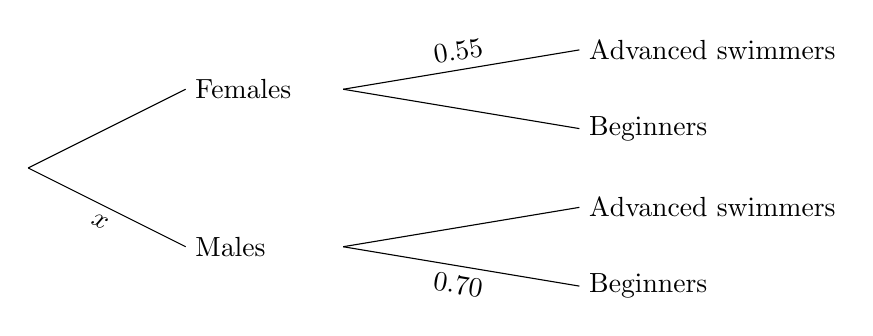
\begin{tikzpicture}
			\draw (0,0) --(2,1) node[right]{Females};
			
			\draw         (4,1) --node[midway,rotate=atan(1/6),above]{$0.55$} (7,1.5) node[right]{Advanced swimmers};
			
			\draw         (4,1) -- (7,0.5) node[right]{Beginners};
			
			\draw (0,0) --node[midway,rotate=-atan(1/2),below]{$x$}(2,-1) node[right]{Males};
			
			\draw         (4,-1) -- (7,-0.5) node[right]{Advanced swimmers};
			
			\draw         (4,-1) --node[midway,rotate=-atan(1/6),below]{$0.70$} (7,-1.5) node[right]{Beginners};
			
		\end{tikzpicture}
	\end{figure*}
	
	For a randomly chosen member, the probability of being an Advanced swimmer is the same as the
	probability of being a Beginner. 
	
	\begin{enumerate}[label=(\roman*)]
		\item Find $x$ \hfill [3]
		\item Given that a randomly chosen member is an Advanced swimmer, find the probability that the
		member is male. \hfill [3]
	\end{enumerate}
	
	
%%%%%%%%%%%%%%%%%%%%%%%%%%%%%%%%%%	
%%%%%%%%%%%%%%%%%%%%%%%%%%%%%%%%%%	
%%%%%%%%%%%%%%%%%%%%%%%%%%%%%%%%%%	
%%%%    Q2 s19_qp_62  q1     %%%	
%%%%%%%%%%%%%%%%%%%%%%%%%%%%%%%%%%	
%%%%%%%%%%%%%%%%%%%%%%%%%%%%%%%%%%	
%%%%%%%%%%%%%%%%%%%%%%%%%%%%%%%%%%		

\item	Two ordinary fair dice are thrown and the numbers obtained are noted. Event $S$ is 'The sum of the numbers is even'. Event $T$ is 'The sum of the numbers is either less than $6$ or a multiple of $4$ or both'. Showing your working, determine whether the events $S$ and $T$ are independent. \hfill  [4]
	
	
	
%%%%%%%%%%%%%%%%%%%%%%%%%%%%%%%%%%	
%%%%%%%%%%%%%%%%%%%%%%%%%%%%%%%%%%	
%%%%%%%%%%%%%%%%%%%%%%%%%%%%%%%%%%	
%%%%    Q3 w17_qp_61  q5     %%%	
%%%%%%%%%%%%%%%%%%%%%%%%%%%%%%%%%%	
%%%%%%%%%%%%%%%%%%%%%%%%%%%%%%%%%%	
%%%%%%%%%%%%%%%%%%%%%%%%%%%%%%%%%%		

\item 	Over a period of time Julian finds that on long-distance flights he flies economy class on $82\%$ of flights. On the rest of the flights he flies first class. When he flies economy class, the probability that he gets a good night's sleep is $x$. When he flies first class, the probability that he gets a good night's
sleep is $0.9$.

\begin{enumerate}[label=(\roman*)]
	\item Draw a fully labelled tree diagram to illustrate this situation. \hfill[2]
\end{enumerate}

The probability that Julian gets a good night's sleep on a randomly chosen flight is $0.285$.

\begin{enumerate}[resume,label=(\roman*)]
	\item Find the value of $x$. \hfill [2]
	\item Given that on a particular flight Julian does not get a good night's sleep, find the probability that he is flying economy class. \hfill [3]
\end{enumerate}
	

%%%%%%%%%%%%%%%%%%%%%%%%%%%%%%%%%%	
%%%%%%%%%%%%%%%%%%%%%%%%%%%%%%%%%%	
%%%%%%%%%%%%%%%%%%%%%%%%%%%%%%%%%%	
%%%%    Q4 w18_qp_61  q7     %%%	
%%%%%%%%%%%%%%%%%%%%%%%%%%%%%%%%%%	
%%%%%%%%%%%%%%%%%%%%%%%%%%%%%%%%%%	
%%%%%%%%%%%%%%%%%%%%%%%%%%%%%%%%%%		

\item In a group of students, the numbers of boys and girls studying Art, Music and Drama are given in the following table. Each of these $160$ students is studying exactly one of these subjects.

\begin{table}[!htpb]
	\centering
	\begin{tabular}{l|c|c|c|}
		\cline{2-4}
		& Art & Music & Drama \\ \hline
		\multicolumn{1}{|l|}{Boys}  & 24  & 40    & 32    \\ \hline
		\multicolumn{1}{|l|}{Girls} & 15  & 12    & 37    \\ \hline
	\end{tabular}
\end{table}

\begin{enumerate}[label=(\roman*)]
	\item Find the probability that a randomly chosen student is studying Music. \hfill[1]
	\item Determine whether the events 'a randomly chosen student is a boy' and 'a randomly chosen
	student is studying Music' are independent, justifying your answer. \hfill [2]
	\item Find the probability that a randomly chosen student is not studying Drama, given that the student	is a girl. \hfill [2]
	\item Three students are chosen at random. Find the probability that exactly $1$ is studying Music and 	exactly $2$ are boys. \hfill  [5]
\end{enumerate}



%%%%%%%%%%%%%%%%%%%%%%%%%%%%%%%%%%	
%%%%%%%%%%%%%%%%%%%%%%%%%%%%%%%%%%	
%%%%%%%%%%%%%%%%%%%%%%%%%%%%%%%%%%	
%%%%    Q5 w18_qp_63  q3    %%%	
%%%%%%%%%%%%%%%%%%%%%%%%%%%%%%%%%%	
%%%%%%%%%%%%%%%%%%%%%%%%%%%%%%%%%%	
%%%%%%%%%%%%%%%%%%%%%%%%%%%%%%%%%%		

\item A box contains $3$ red balls and $5$ blue balls. One ball is taken at random from the box and not replaced. A yellow ball is then put into the box. A second ball is now taken at random from the box.

\begin{enumerate}[label=(\roman*)]
	\item  Complete the tree diagram to show all the outcomes and the probability for each branch. \hfill[2]
	
	\begin{figure*}[!htpb]
		\centering
		\begin{tikzpicture}
			\draw (0,0) --(2,1.5);
			
			\draw         (4,1.5) -- (7,2.5);
			
			\draw         (4,1.5) -- (7,1.5);
			\draw         (4,1.5) -- (7,0.5);
			
		\draw (0,0) --(2,-1.5);
		
		\draw         (4,-1.5) -- (7,-2.5);
		
		\draw         (4,-1.5) -- (7,-1.5);
		\draw         (4,-1.5) -- (7,-0.5);
		
		\node at (3,3.5) {First ball};
		\node at (8,3.5) {Second ball};
			
		\end{tikzpicture}
	\end{figure*}



\item  Find the probability that the two balls taken are the same colour.  \hfill[2]

\item  Find the probability that the first ball taken is red, given that the second ball taken is blue. \hfill [3]




\end{enumerate}


%%%%%%%%%%%%%%%%%%%%%%%%%%%%%%%%%%	
%%%%%%%%%%%%%%%%%%%%%%%%%%%%%%%%%%	
%%%%%%%%%%%%%%%%%%%%%%%%%%%%%%%%%%	
%%%%    Q6 w16_qp_61  q6    %%%	
%%%%%%%%%%%%%%%%%%%%%%%%%%%%%%%%%%	
%%%%%%%%%%%%%%%%%%%%%%%%%%%%%%%%%%	
%%%%%%%%%%%%%%%%%%%%%%%%%%%%%%%%%%		

\item Deeti has $3$ red pens and $1$ blue pen in her left pocket and $3$ red pens and $1$ blue pen in her right pocket. 'Operation $T$' consists of Deeti taking one pen at random from her left pocket and placing it in her right pocket, then taking one pen at random from her right pocket and placing it in her left pocket.

\begin{enumerate}[label=(\roman*)]
	\item Find the probability that, when Deeti carries out operation $T$, she takes a blue pen from her left pocket and then a blue pen from her right pocket. \hfill[2]
\end{enumerate}

The random variable $X$ is the number of blue pens in Deeti's left pocket after carrying out operation $T$.

\begin{enumerate}[resume,label=(\roman*)]
	\item Find P($X$) = $1$. \hfill[3]
	\item Given that the pen taken from Deeti's right pocket is blue, find the probability that the pen taken
	from Deeti's left pocket is blue. \hfill [4]
\end{enumerate}


%%%%%%%%%%%%%%%%%%%%%%%%%%%%%%%%%%	
%%%%%%%%%%%%%%%%%%%%%%%%%%%%%%%%%%	
%%%%%%%%%%%%%%%%%%%%%%%%%%%%%%%%%%	
%%%%    Q7 m16_qp_62  q3    %%%	
%%%%%%%%%%%%%%%%%%%%%%%%%%%%%%%%%%	
%%%%%%%%%%%%%%%%%%%%%%%%%%%%%%%%%%	
%%%%%%%%%%%%%%%%%%%%%%%%%%%%%%%%%%		

\item A fair eight-sided die has faces marked $1$, $2$, $3$, $4$, $5$, $6$, $7$, $8$. The score when the die is thrown is the number on the face the die lands on. The die is thrown twice.

\begin{itemize}
	\setlength\itemsep{0.5em}
	\item Event $R$ is 'one of the scores is exactly $3$ greater than the other score'.
	\item Event $S$ is 'the product of the scores is more than $19$'.
\end{itemize}

\begin{enumerate}[label=(\roman*)]
	\item Find the probability of $R$. \hfill[2]
	\item Find the probability of $S$. \hfill[2]
	\item Determine whether events $R$ and $S$ are independent. Justify your answer. \hfill[3]
\end{enumerate}

%%%%%%%%%%%%%%%%%%%%%%%%%%%%%%%%%%	
%%%%%%%%%%%%%%%%%%%%%%%%%%%%%%%%%%	
%%%%%%%%%%%%%%%%%%%%%%%%%%%%%%%%%%	
%%%%    Q8 s15_qp_61  q3    %%%	
%%%%%%%%%%%%%%%%%%%%%%%%%%%%%%%%%%	
%%%%%%%%%%%%%%%%%%%%%%%%%%%%%%%%%%	
%%%%%%%%%%%%%%%%%%%%%%%%%%%%%%%%%%		

\item Jason throws two fair dice, each with faces numbered $1$ to $6$. Event A is 'one of the numbers obtained
is divisible by $3$ and the other number is not divisible by $3$'. Event $B$ is 'the product of the two
numbers obtained is even'.

\begin{enumerate}[label=(\roman*)]
	\item Determine whether events $A$ and $B$ are independent, showing your working.  \hfill[5]
	\item Are events $A$ and $B$ mutually exclusive? Justify your answer. \hfill[1]
\end{enumerate}

\newpage 
%%%%%%%%%%%%%%%%%%%%%%%%%%%%%%%%%%	
%%%%%%%%%%%%%%%%%%%%%%%%%%%%%%%%%%	
%%%%%%%%%%%%%%%%%%%%%%%%%%%%%%%%%%	
%%%%    Q9 s15_qp_63  q2    %%%	
%%%%%%%%%%%%%%%%%%%%%%%%%%%%%%%%%%	 
%%%%%%%%%%%%%%%%%%%%%%%%%%%%%%%%%%	
%%%%%%%%%%%%%%%%%%%%%%%%%%%%%%%%%%		

\item	When Joanna cooks, the probability that the meal is served on time is $\frac{1}{5}$. The probability that the
kitchen is left in a mess is $\frac{3}{5}$. The probability that the meal is not served on time and the kitchen is not
left in a mess is $\frac{3}{10}$. Some of this information is shown in the following table.


\medskip

\begin{table}[!htpb]
	\centering
	\begin{tabular}{l|c|c|c|}
		\cline{2-4}
		& Kitchen left in a mess & Kitchen left not in a mess & Total \\ \hline
		\multicolumn{1}{|l|}{Meal served on time}     &                        &                            &   $\frac{1}{5}$    \\ \hline
		\multicolumn{1}{|l|}{Meal not served on time} &                        &                  $\frac{3}{10}$          &       \\ \hline
		\multicolumn{1}{|l|}{Total}                   &                        &                            & 1     \\ \hline
	\end{tabular}
\end{table}

\begin{enumerate}[label=(\roman*)]
	\item Copy and complete the table. \hfill[3]
	\item Given that the kitchen is left in a mess, find the probability that the meal is not served on time. 
	
	
	\,\quad 
	\hfill 
	[2]
\end{enumerate}


%%%%%%%%%%%%%%%%%%%%%%%%%%%%%%%%%%	
%%%%%%%%%%%%%%%%%%%%%%%%%%%%%%%%%%	
%%%%%%%%%%%%%%%%%%%%%%%%%%%%%%%%%%	
%%%%    Q10 s14_qp_63  q6    %%%	
%%%%%%%%%%%%%%%%%%%%%%%%%%%%%%%%%%	
%%%%%%%%%%%%%%%%%%%%%%%%%%%%%%%%%%	
%%%%%%%%%%%%%%%%%%%%%%%%%%%%%%%%%%		

\item Tom and Ben play a game repeatedly. The probability that Tom wins any game is $0.3$. Each game is
won by either Tom or Ben. Tom and Ben stop playing when one of them (to be called the champion)
has won two games.

\begin{enumerate}[label=(\roman*)]
	\item Find the probability that Ben becomes the champion after playing exactly $2$ games. \hfill [1]
	
	\item Find the probability that Ben becomes the champion.  \hfill[3]
	\item Given that Tom becomes the champion, find the probability that he won the $2$nd game. \hfill[4]
\end{enumerate}



	
\end{enumerate}

	

	
	
	
	
	



